\textcolor{principal}{M\'ETODO DE VALUACI\'ON POR CAPITALIZACI\'ON DIRECTA. }\\

\textcolor{principal}{Capitalizaci\'on mediante Perpetuidad Creciente.} \\

El valuador requiere determinar un pron\'ostico de flujo neto (despu\'es de impuestos), para el negocio, conocido como \textcolor{principal}{Free Cash Flow to Equity \textit{(\gls{fcfe})}}, el cual se capitaliza a una tasa financiera que involucra una estimaci\'on de costo de capital como rentabilidad m\'inima esperada para los accionistas v\'ia dividendos, as\'i como el crecimiento del valor del capital contable de un negocio como plusval\'ia.


\begin{center}
\begin{figure}[H]
\centering
\begin{minipage}{8cm}
\centering
	\caption{Capitalizaci\'on Directa mediante perpetuidad creciente\label{fig:cap_dir}}
	
	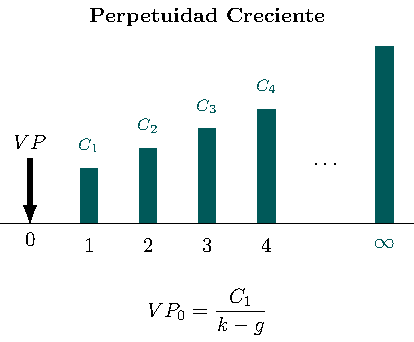
\includegraphics[width=5cm]{\rutaImagenes/capitalizacion_directa}
	\end{minipage}
	 \hspace{1pt} \begin{minipage}{5cm}
	Donde:
	\begin{itemize}
	
		\item $C_1$: Flujo de caja
		\item $k$: Tasa de Capitalizaci\'on
		\item $g$: Tasa de Crecimiento
	\end{itemize}
	\end{minipage}
\end{figure}
\end{center}



